% ============================================================================
%  Colour alone as an early trigger for strongly lensed Type Ia supernovae
%  MNRAS-style draft. Compile on Overleaf (mnras.cls is built in) or with a
%  local TeX Live that has mnras.cls:  pdflatex paper; bibtex paper; pdflatex x2
% ============================================================================
\documentclass[fleqn,usenatbib]{mnras}

\usepackage{newtxtext,newtxmath}   % MNRAS-recommended fonts (drop if unavailable)
\usepackage[T1]{fontenc}
\usepackage{graphicx}
\usepackage{amsmath}
\usepackage{booktabs}
\usepackage{siunitx}

\graphicspath{{figures/}}

% ---- convenience macros -----------------------------------------------------
\newcommand{\ugrizy}{\textit{ugrizy}}
\newcommand{\gr}{$g\!-\!r$}
\newcommand{\zy}{$z\!-\!y$}
\newcommand{\iz}{$i\!-\!z$}
\newcommand{\Msun}{\mathrm{M}_\odot}

\title[Colour as an early trigger for lensed SNe~Ia]{Colour alone as an early
trigger for strongly lensed Type~Ia supernovae in the Rubin/LSST survey}

% --- PLACEHOLDER author block: fill in real names, affiliations and e-mail ---
\author[Author et al.]{
A.~N.~Author,$^{1}$\thanks{E-mail: your.email@example.com}
B.~Coauthor$^{1}$
and C.~Supervisor$^{1}$
\\
$^{1}$\textit{School of Physics and Astronomy, University of Birmingham,
Edgbaston, Birmingham B15 2TT, UK}
}

\date{Draft \today}
\pubyear{2026}

\begin{document}
\label{firstpage}
\maketitle

% =============================================================================
\begin{abstract}
Strongly lensed Type~Ia supernovae (SNe~Ia) are rare but powerful probes of
$H_0$ and of lens mass distributions, and their value is greatest when the
system is flagged early---before the trailing image appears. We ask whether
\emph{colour alone}, with no host photometric redshift and no spectroscopy, can
act as such an early trigger in the Rubin Observatory Legacy Survey of Space and
Time (LSST). Using the \textsc{cmsne} pipeline we generate SN~Ia and four
core-collapse (CC) contaminant classes---each lensed and unlensed---through a
realistic OpSim cadence, weight every class by its literature-anchored
volumetric rate, and train a missing-data-native gradient-boosted classifier on
the \ugrizy\ colour vector. We find that (i) the optimal decision boundary
between lensed and unlensed populations is a smooth \emph{gradient} rather than a
sharp line, so candidates should be ranked by a calibrated probability rather
than hard-cut; (ii) although CC intrinsically outnumber SNe~Ia $\sim\!3\!:\!1$,
the flux-limited \emph{detected} background is $\sim$70\% unlensed SNe~Ia and
$\sim$30\% CC, making the colour-identical unlensed SN~Ia the irreducible
contaminant; (iii) under a real cadence the full colour vector is essential---one
fixed colour recovers only 11\% of lensed SNe~Ia at 10\% contamination whereas
using whatever bands are present recovers 32--48\%; (iv) the trigger flags 56\%
of lensed SNe~Ia a median of $\sim$3\,d after first detection and, when it flags
a system, beats the second image 85\% of the time with a median lead of 88\,d;
(v) at the true base rate ($\sim$1 in $10^4$) the flagged sample is sub-percent
pure, so colour is a strong \emph{pre-filter} (cutting the follow-up list
$\sim$40$\times$) rather than a standalone identifier. The results are stable
across two OpSim baselines (v5.3.2 and v5.3.5). We release the pipeline, the
classifier, and a demonstration notebook.
\end{abstract}

\begin{keywords}
gravitational lensing: strong -- supernovae: general -- methods: statistical --
surveys
\end{keywords}

% =============================================================================
\section{Introduction}
\label{sec:intro}

Strongly lensed supernovae are among the most information-rich transients in
time-domain astronomy. The relative time delays between multiple images provide
a one-step, largely geometric measurement of the Hubble constant
\citep{Refsdal1964,Suyu2020}, and lensed SNe~Ia additionally benefit from the
standardisable luminosity of their source, breaking degeneracies that limit
lensed-quasar cosmography. Only a handful are known---the cluster-lensed
SN~Refsdal \citep{Kelly2015} and the galaxy-lensed SN~Ia iPTF16geu
\citep{Goobar2017}---but the Rubin Observatory Legacy Survey of Space and Time
\citep[LSST;][]{Ivezic2019} is forecast to discover of order ten lensed SNe~Ia
per year \citep{Oguri2010,Goldstein2019,Wojtak2019}.

Realising their cosmological value requires catching the delayed images, which
in turn requires flagging a candidate \emph{early}---ideally from the leading
image, before the system is recognisably multiple. This is difficult:
gravitational magnification is achromatic, so a lensed SN~Ia is photometrically a
normal, if unusually bright, SN~Ia and leaves no colour imprint of lensing
itself. What colour \emph{can} do is \emph{type} a transient---separate a SN~Ia
from the core-collapse (CC) background---cheaply and early, from whatever bands a
survey has measured, without a host redshift.

In this paper we test, end to end, whether colour alone can serve as an early
trigger for lensed SNe~Ia in LSST. We deliberately exclude any redshift-based
feature (such as comparing an observed magnitude to the expected unlensed
magnitude at a known redshift): powerful though these are, they defeat the
purpose of a photometry-only trigger. Section~\ref{sec:method} describes the
simulation, rate model, features, and classifier. Section~\ref{sec:results}
presents the results: the shape of the optimal decision boundary, the true
composition of the detected background, the recovery achievable under a real
cadence, the ``colour-first'' lead over the second image, the sobering
base-rate purity, robustness across survey baselines, and a comparison of
brightness features. We discuss limitations in Section~\ref{sec:discussion} and
conclude in Section~\ref{sec:conclusions}.

% =============================================================================
\section{Method}
\label{sec:method}

\subsection{Transient populations and lensing}
\label{sec:populations}

We simulate five source classes: SNe~Ia, modelled with SALT3
\citep{Kenworthy2021}, and four CC templates
(\texttt{nugent-sn1bc}, \texttt{-sn2l}, \texttt{-sn2n}, \texttt{-sn2p};
\citealt{Nugent2002}), each in an unlensed and a strongly lensed variant---ten
populations in total. Peak absolute magnitudes and scatters for the CC templates
follow measured luminosity functions.

Strong lensing is applied with a four-component magnification model: galaxy-,
group-, and cluster-scale lenses adopt a $(\mu/4)^{-3}$ magnification-dependent
time-delay prefactor and a fourth population uses $(\mu/4)^{-1}$, where $\mu$ is
the total magnification. The strong-lensing optical depth scales as
$(d/31\,\mathrm{Gpc})^{3}\,\mu^{-2}$, so high-magnification, most
signal-like configurations are strongly suppressed. Observer-frame observation
times are converted to the rest frame by dividing by $(1+z)$ where the model
requires it, whereas magnitudes are never redshift-divided.

\subsection{Volumetric rates and cross-class weighting}
\label{sec:rates}

Every event enters the rate-weighted statistics with a weight equal to the
integral of its class's volumetric rate over the sampled redshift (and, for
lensed classes, magnification) range. The SN~Ia rate follows a
\citet{Madau2014} star-formation history convolved with a delay-time
distribution; the CC rate tracks the star-formation history directly.

Because the SN~Ia and CC rate grids carry independent normalisations, a single
constant sets the cross-class balance. We anchor it to the local literature: a
SN~Ia volumetric rate $\sim\!2.4\times10^{-5}\,\mathrm{yr}^{-1}\,\mathrm{Mpc}^{-3}$
\citep{Frohmaier2019} and a CC rate
$\sim\!7\times10^{-5}\,\mathrm{yr}^{-1}\,\mathrm{Mpc}^{-3}$
\citep{Li2011,Taylor2014}, i.e.\ CC:Ia~$\approx3\!:\!1$ locally. The redshift
evolution of the ratio then follows the star-formation-history (CC) and
delay-time-distribution (Ia) shapes. The four CC sub-types are further weighted
by realistic volumetric fractions
(Ib/c 0.36, II-P 0.55, II-n 0.06, II-L 0.03; \citealt{Li2011,Shivvers2017}) so
that the luminous but rare SN~IIn does not carry the same weight as the common
SN~IIP.

\subsection{Survey simulation and detection}
\label{sec:cadence}

Light curves are realised through a real LSST cadence using OpSim visit
histories, with per-band single-visit limiting magnitudes as the detection
threshold. The production results use the \texttt{baseline\_v5.3.2} cadence;
\texttt{v5.3.5} is used as an independent robustness check
(Section~\ref{sec:robustness}). An event is ``detected'' once it clears the
threshold in at least one visit. For every detected event we record the full
colour vector at the trigger (first-detection) epoch and at a short evolution
baseline thereafter.

\subsection{Colour and brightness features}
\label{sec:features}

The feature vector is the five adjacent-band colours
$u\!-\!g,\,g\!-\!r,\,r\!-\!i,\,i\!-\!z,\,z\!-\!y$, optionally augmented by their
short-baseline evolution and by a single apparent-brightness feature. Crucially,
at first detection a real cadence rarely delivers a \emph{specific} colour: \gr\
is present only $\sim$9\% of the time, and $\sim$48\% of detected events have
just one band (no colour at all). The features are therefore treated as
missing-data-native, so the method uses whatever bands are present rather than
committing to one fixed colour. For the brightness feature we record three
candidates and compare them in Section~\ref{sec:magfeature}.

\subsection{Classifier and decision boundary}
\label{sec:classifier}

The classifier is a histogram-based gradient-boosted decision tree
(\citealt{Pedregosa2011}; NaN-native, so missing colours need no imputation) on
the colour vector, rate-weighted, with the signal up-weighted to a balanced
training prior. Scores are isotonic-calibrated, and an optional hard decision
threshold is pinned to a target rate-weighted contamination (default 10\%). The
classifier exposes a calibrated posterior $P(\text{lensed}\mid\text{colour})$
that folds in the true base rate through a likelihood-ratio update, and a
ranking interface---reflecting the finding
(Section~\ref{sec:gradient}) that the lensed/unlensed transition is a broad
gradient and candidates should be ranked, not hard-cut.

\subsection{Evaluation metrics}
\label{sec:metrics}

Our primary metric is \emph{recovery at fixed contamination}: the rate-weighted
fraction of lensed SNe~Ia retained when only one survivor in ten is a
contaminant (recovery at 10\% false-positive rate). We also report ROC-AUC, the
\emph{colour-first} fraction (whether the trigger fires before the second image
becomes detectable, i.e.\ before one lensing time delay), the median lead time,
and---at the true base rate---the purity and the follow-up cost (candidates to
vet per genuine lensed SN~Ia).

% =============================================================================
\section{Results}
\label{sec:results}

\subsection{The decision boundary is a gradient, not a line}
\label{sec:gradient}

Framing the problem correctly---signal $=$ lensed SNe~Ia, background $=$ unlensed
SNe~Ia plus all CC classes (lensed and unlensed), rate-weighted---we compare six
boundary families against the same features (Fig.~\ref{fig:boundary}). The
current straight-line boundary recovers $\sim$63\% of lensed SNe~Ia at 10\%
contamination, whereas a kernel-density ratio, a decision tree, and even a simple
per-magnitude step or sloped step all reach $\sim$88--89\%. Any flexible boundary
beats the line, and the elaborate two-dimensional tree is barely ahead of a
simple step once the rates are realistic. Fig.~\ref{fig:problem} shows the two
populations across all ten band pairs: the lensed SNe~Ia are a sparse signal
embedded in the dense contaminant background, well separated for blue baselines
(tree AUC $\sim$0.9--0.96) and increasingly overlapped toward the red (\zy\ AUC
$\sim$0.83).

\begin{figure*}
  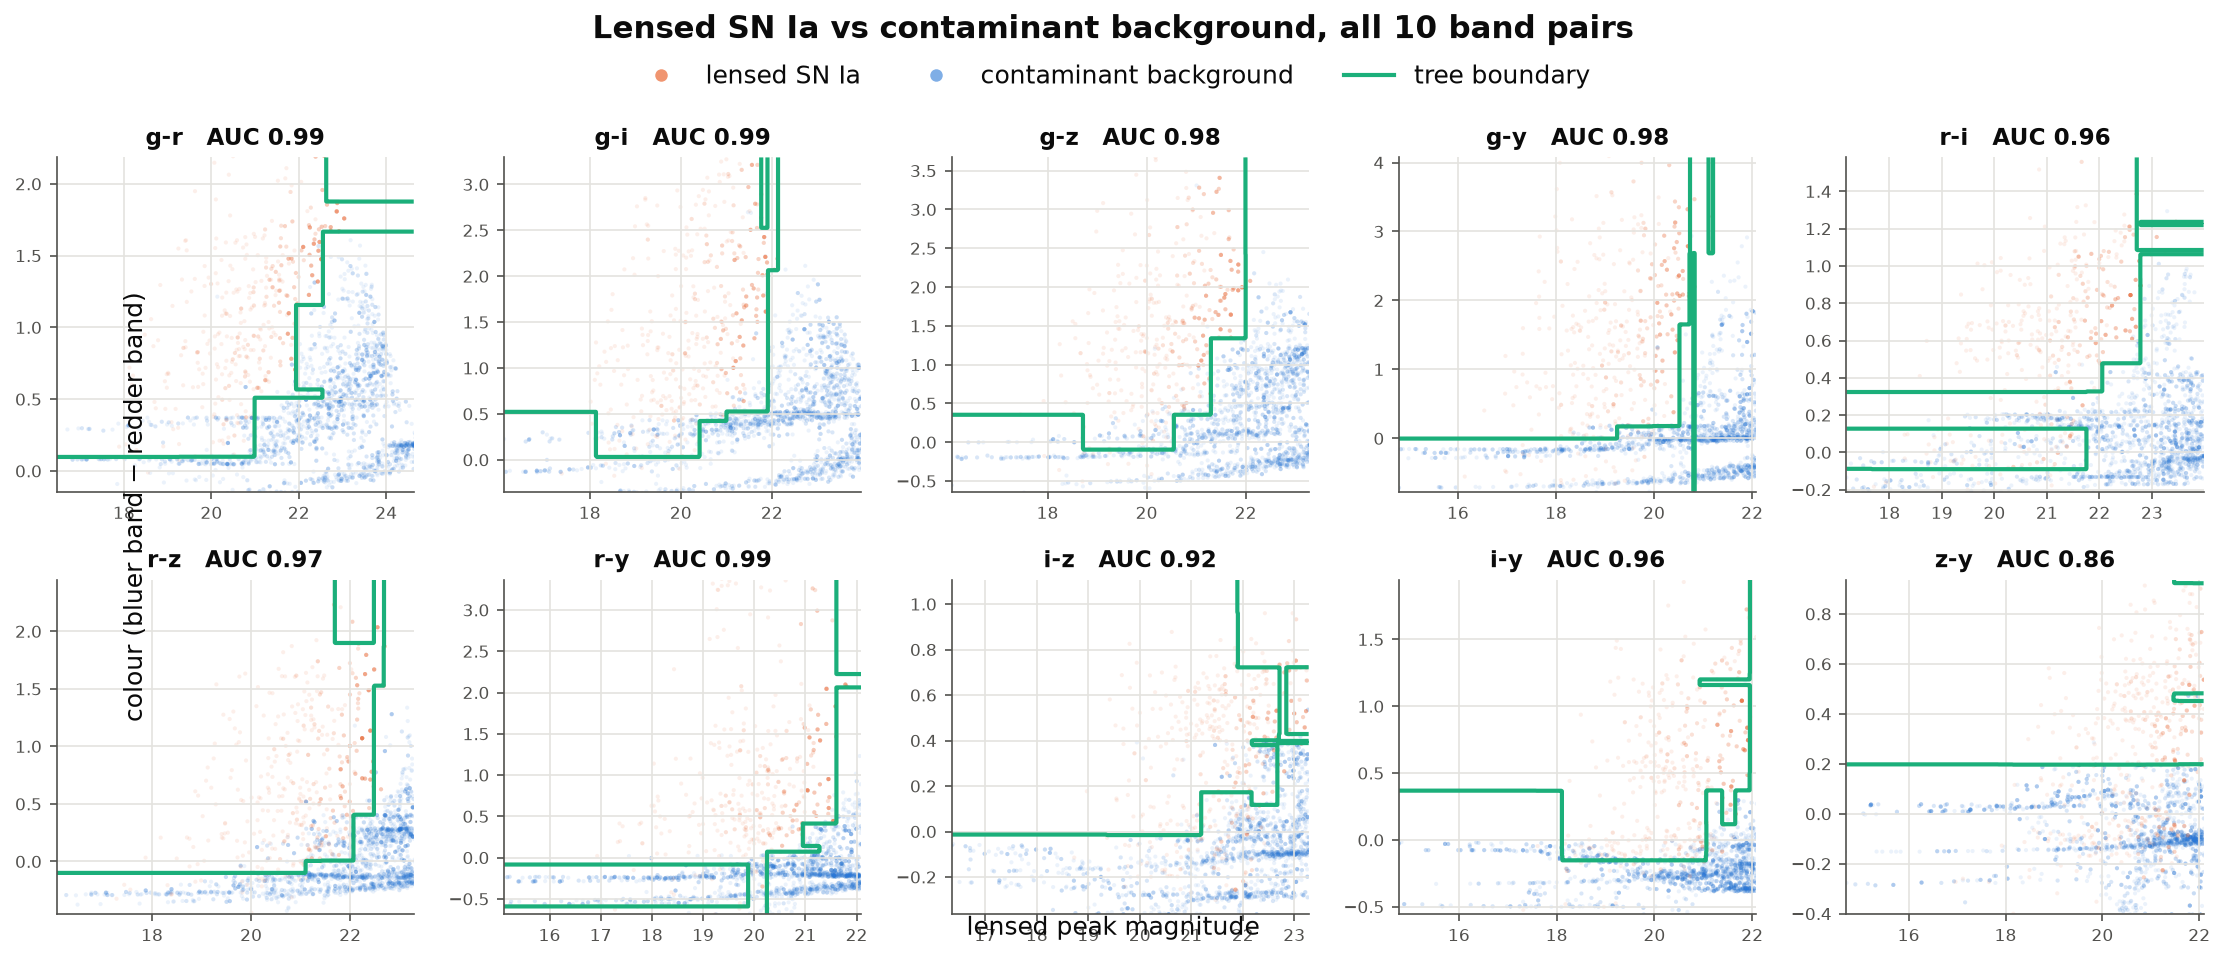
\includegraphics[width=\textwidth]{gal_cmd}
  \caption{The classification problem in all ten colour--magnitude planes. Lensed
  SNe~Ia (orange) are a sparse signal embedded in the dense contaminant
  background (blue) of unlensed SNe~Ia and core-collapse SNe. Separability is best
  for blue baselines and collapses for the reddest, most overlapped pair (\zy).}
  \label{fig:problem}
\end{figure*}

The underlying posterior $P(\text{lensed}\mid\text{colour},\text{magnitude})$ is
smooth (Fig.~\ref{fig:gradient}): its $P=0.5$ ridge is a clean diagonal and the
transition is broad, with the ambiguous $0.2<P<0.8$ band holding $\sim$11--14\%
of rate-weighted events for blue pairs but 40\% for \iz\ and 48\% for \zy. The
operational recommendation, implemented in the pipeline, is to report the
calibrated probability and rank candidates rather than apply a hard cut.

\begin{figure}
  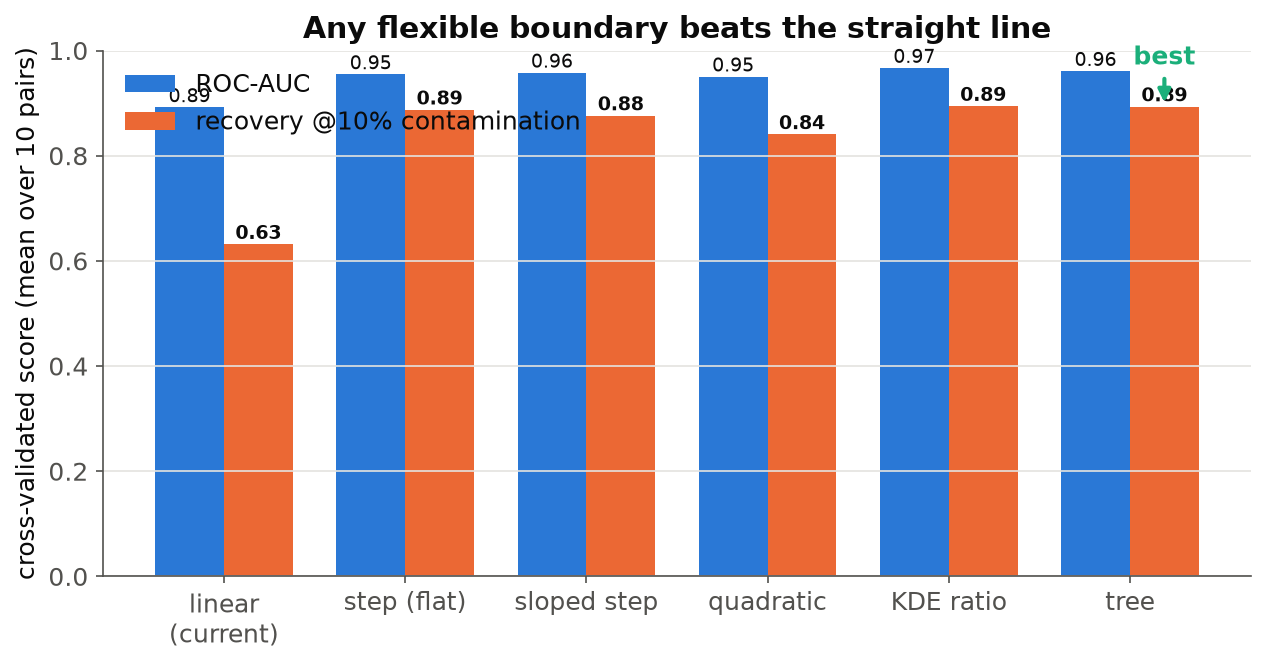
\includegraphics[width=\columnwidth]{bd_compare}
  \caption{Recovery of lensed SNe~Ia at 10\% contamination for six decision-boundary
  families. The straight line ($\sim$0.63) is beaten by every flexible boundary;
  a kernel-density ratio, a decision tree, and a simple per-magnitude step all
  reach $\sim$0.88--0.89. Once the rate weighting is realistic, elaborate
  two-dimensional structure adds little over a simple discontinuous step.}
  \label{fig:boundary}
\end{figure}

\begin{figure}
  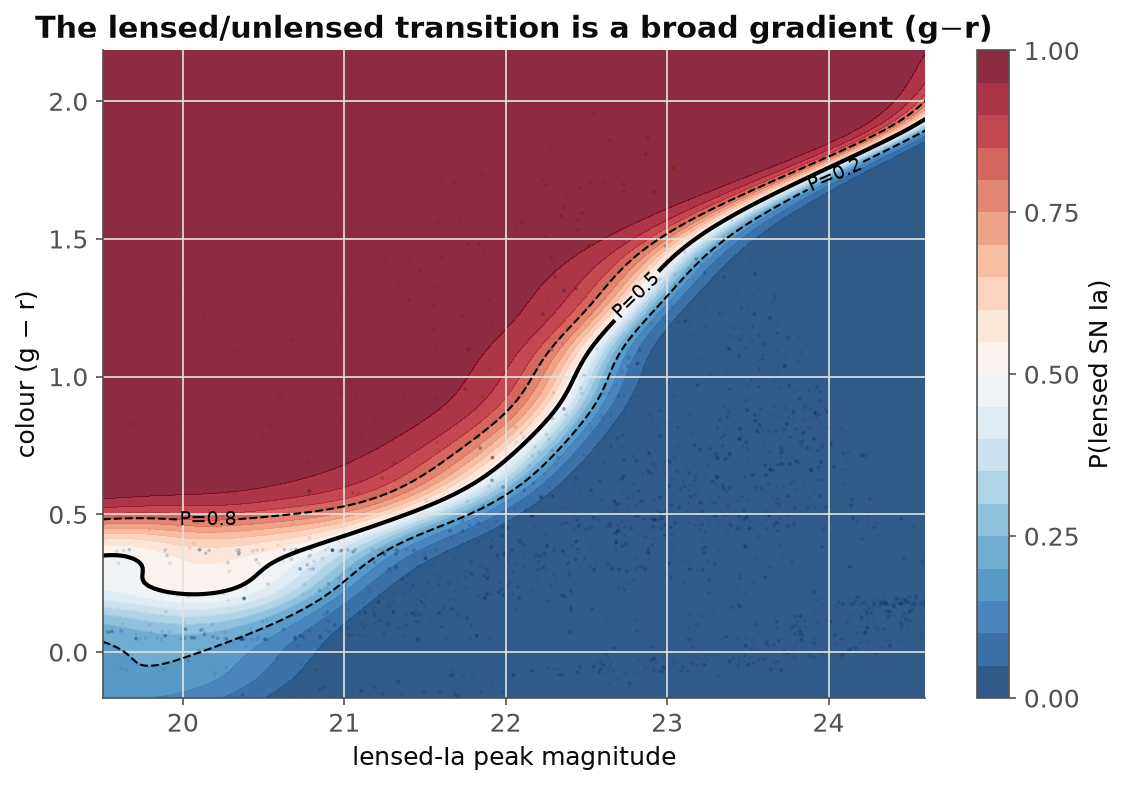
\includegraphics[width=\columnwidth]{grad_field}
  \caption{The calibrated posterior $P(\text{lensed}\mid\text{colour},
  \text{magnitude})$ is a smooth gradient. The $P=0.5$ contour is a clean
  diagonal and the transition is broad---especially for red band pairs---so the
  right output is a ranked probability, not a hard cut.}
  \label{fig:gradient}
\end{figure}

\subsection{The detected background is SN\,Ia-dominated}
\label{sec:composition}

Although CC intrinsically outnumber SNe~Ia $\sim3\!:\!1$
(Section~\ref{sec:rates}), the \emph{detected} background is the opposite
(Fig.~\ref{fig:composition}). Flux-limited detection favours the brighter
SNe~Ia, seen to larger volume, and the realistic sub-type mix down-weights the
luminous-but-rare SN~IIn. Rate-weighted and restricted to detected events, the
contaminant background is $\sim$70\% unlensed SNe~Ia, $\sim$30\% CC, with lensed
CC utterly negligible ($\sim\!10^{-3}$\%).

The consequence is important: the dominant contaminant is the colour-identical
unlensed SN~Ia, which magnification cannot distinguish by colour. Multi-colour
therefore earns its keep in two ways---cleanly rejecting the $\sim$30\% CC, and
exploiting the mild reddening and extra brightness of the higher-redshift lensed
Ia---while the lensing verdict itself is deferred to a later,
brightness/multiplicity/spectroscopy-based stage.

\begin{figure}
  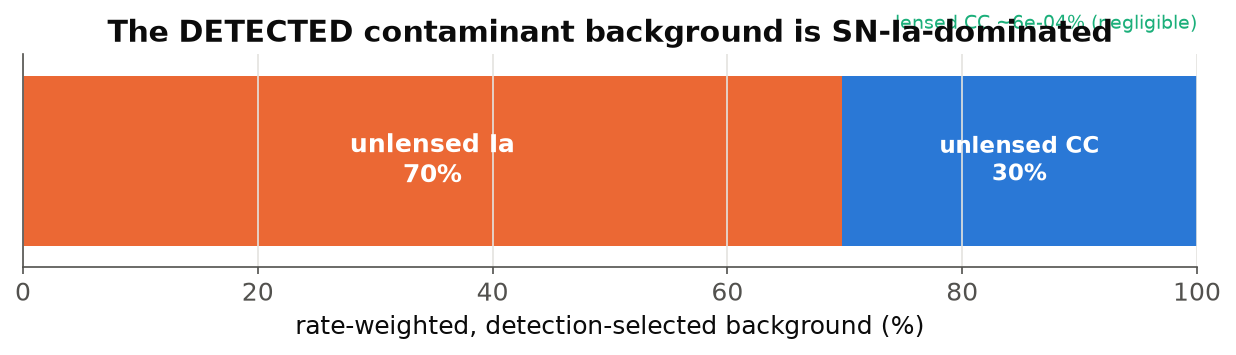
\includegraphics[width=\columnwidth]{bd_composition}
  \caption{The rate-weighted, detection-selected contaminant background is
  SN\,Ia-dominated: $\sim$70\% unlensed SNe~Ia, $\sim$30\% core-collapse, and
  lensed core-collapse negligible. The colour-identical unlensed SNe~Ia are the
  irreducible contaminant that colour cannot remove.}
  \label{fig:composition}
\end{figure}

\subsection{Under a real cadence, multi-colour is essential}
\label{sec:multicolour}

In the idealised limit (every band measured at peak), colour-only recovery of
lensed SNe~Ia rises from $\sim$0.40 (one colour) to $\sim$0.98 (all five
\ugrizy\ colours), and five colours alone match colour$+$magnitude. Under a real
cadence at first detection, where a specific colour is usually missing, the
picture is more sobering but the ranking is unchanged (Fig.~\ref{fig:recovery};
Table~\ref{tab:recovery}). The value of multi-colour is \emph{band
redundancy}: a single fixed colour is missing nine times out of ten at first
light, so the trigger must use the bands it happens to have. A first-detection
trigger sees only $\sim$2 bands, which caps recovery near 0.5.

\begin{figure}
  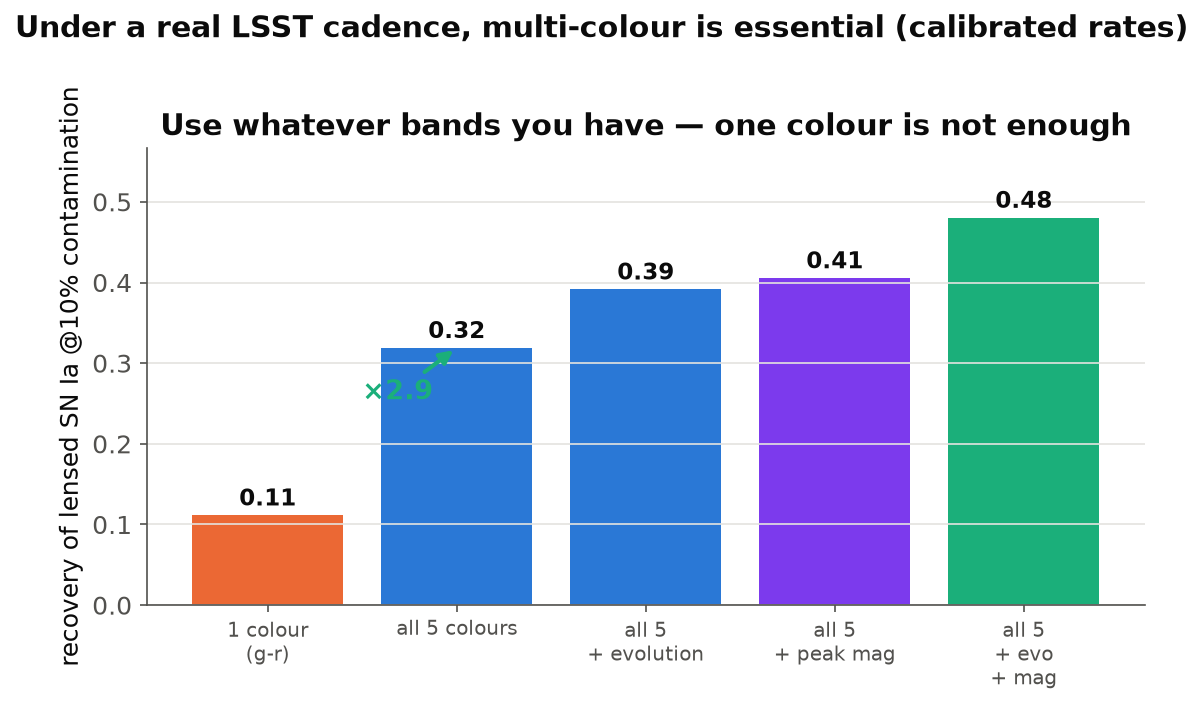
\includegraphics[width=\columnwidth]{mc_recovery}
  \caption{Cadence-realistic recovery of lensed SNe~Ia at 10\% contamination.
  Committing to one fixed colour (\gr) recovers only 0.11; using whatever bands
  are present triples it, colour evolution and the peak magnitude add more.
  Multi-colour's practical value is band redundancy.}
  \label{fig:recovery}
\end{figure}

\begin{table}
  \centering
  \caption{Cadence-realistic recovery of lensed SNe~Ia at 10\% contamination
  (calibrated rates, v5.3.2). ``+ evolution'' adds the short-baseline colour
  change; the magnitude feature is the brightest observed sample
  (Section~\ref{sec:magfeature}).}
  \label{tab:recovery}
  \begin{tabular}{lc}
    \toprule
    feature set & recovery @10\% contam. \\
    \midrule
    1 fixed colour (\gr)     & 0.11 \\
    all 5 colours            & 0.32 \\
    all 5 $+$ evolution      & 0.39 \\
    all 5 $+$ peak magnitude & 0.41 \\
    all 5 $+$ evolution $+$ magnitude & \textbf{0.48} \\
    \bottomrule
  \end{tabular}
\end{table}

\subsection{Waiting a few weeks lifts recovery, then plateaus}
\label{sec:waiting}

Waiting after first detection to accumulate more bands roughly doubles recovery
and then flattens (Fig.~\ref{fig:waiting}): colour-only recovery goes 0.28
(3\,d) $\rightarrow$ 0.47 (30\,d) $\rightarrow$ 0.49 (60\,d), reaching $\sim$0.56
by 60\,d with the peak magnitude included. The yield of lensed SNe~Ia with at
least one colour rises from 31\% (3\,d) to 62\% (30\,d) and plateaus near 65\%:
about a third of lensed SNe~Ia are only ever seen in a single band, an
irreducible cadence limit. The practical sweet spot is $\sim$2--4 weeks after
first light.

\begin{figure}
  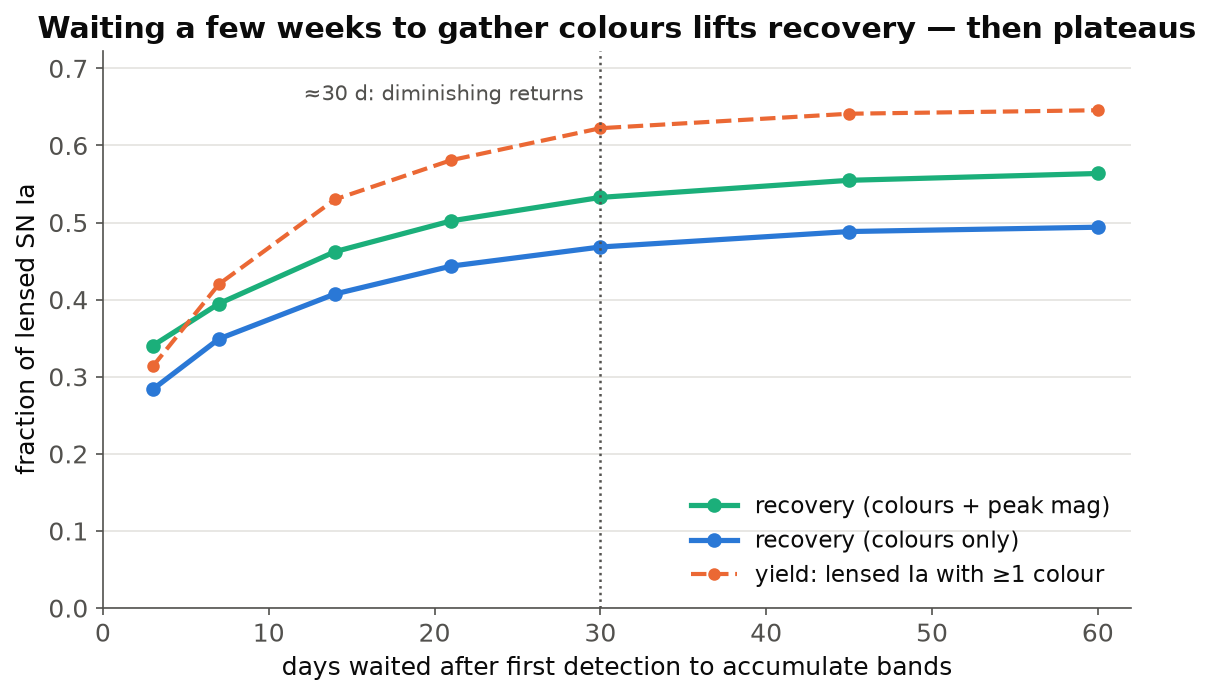
\includegraphics[width=\columnwidth]{mc_waiting}
  \caption{Recovery and yield as a function of the time waited after first
  detection to accumulate bands. Recovery roughly doubles by $\sim$30\,d and then
  plateaus; a third of lensed SNe~Ia are only ever seen in one band.}
  \label{fig:waiting}
\end{figure}

\subsection{Colour-first: the trigger beats the second image}
\label{sec:colourfirst}

The central science question is whether the colour trigger fires before the
second image becomes detectable, roughly one time delay later. Packaging the
features into the classifier, the multi-colour identifier flags 56\% of lensed
SNe~Ia, fires a median of $\sim$3\,d after first detection, and---when it flags a
system---beats the second image 85\% of the time by a median of 88\,d
(Fig.~\ref{fig:colourfirst}). That large lead is the argument for a colour-only
trigger: it flags the majority of lensed SNe~Ia, early, from photometry alone.

\begin{figure*}
  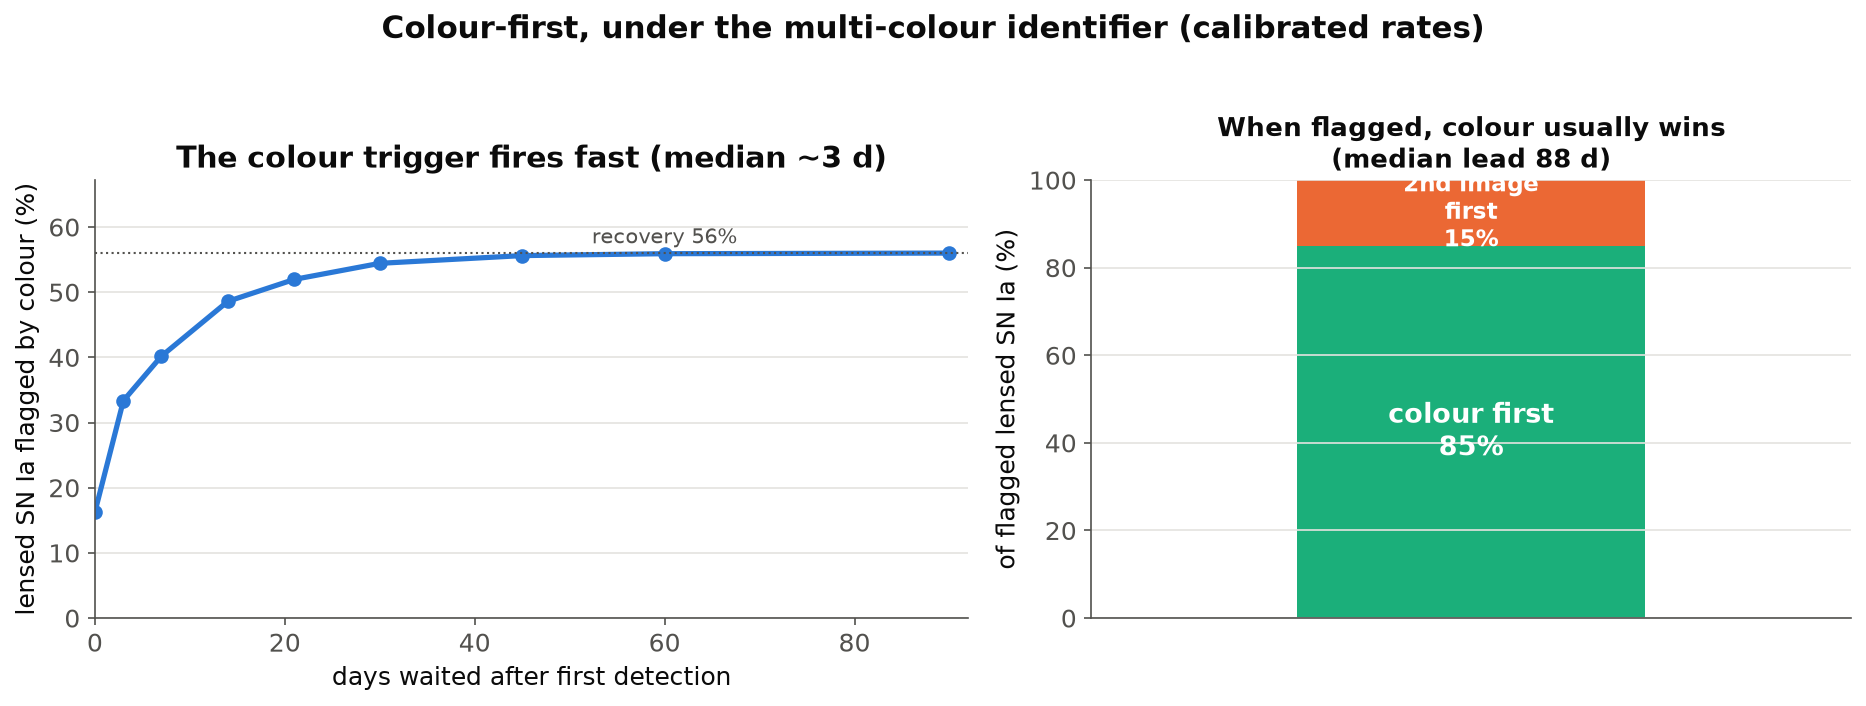
\includegraphics[width=\textwidth]{mc_colourfirst}
  \caption{Left: the cumulative fraction of lensed SNe~Ia flagged by the colour
  trigger as a function of time since first detection; the trigger fires fast
  (median $\sim$3\,d). Right: of the flagged systems, the fraction for which
  colour beats the second image (85\%), with a median lead of 88\,d.}
  \label{fig:colourfirst}
\end{figure*}

\subsection{The base rate is brutal: colour is a pre-filter}
\label{sec:baserate}

At the literature prior ($\sim$9 lensed SNe~Ia\,yr$^{-1}$ against $\sim$10$^5$
detected SNe\,yr$^{-1}$, i.e.\ $\sim$1 in $10^4$), even the multi-colour
identifier gives sub-0.1\% purity at useful recovery: flagging half the lensed
SNe~Ia yields a sample only $\sim$0.03\% real (Fig.~\ref{fig:baserate}). What
colour \emph{does} buy is a drastic cut in the follow-up list---from $\sim$10\,000
detected SNe per genuine lensed Ia (no filter) to a few hundred at tight
recovery, a $\sim$40$\times$ reduction. Colour is thus a strong
\emph{prioritiser} feeding a second stage, and should be scored by purity or
follow-up cost at the true prior rather than by balanced accuracy.

\begin{figure*}
  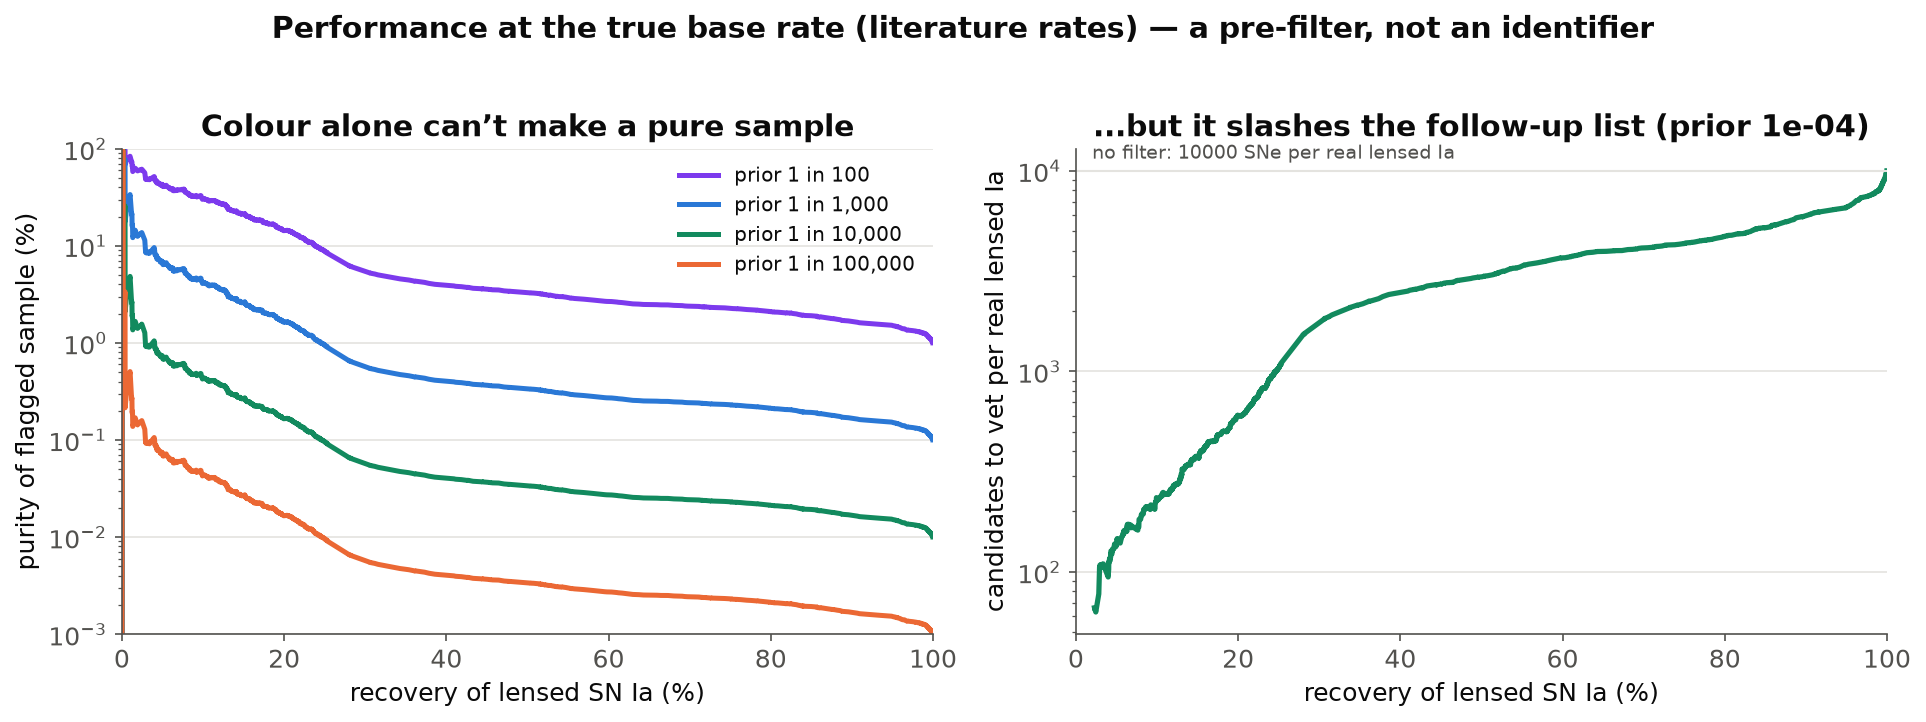
\includegraphics[width=\textwidth]{mc_baserate}
  \caption{Left: purity of the flagged sample as a function of recovery, for
  priors from 1 in $10^2$ to 1 in $10^5$; at the literature prior ($\sim$1 in
  $10^4$) the sample is sub-percent pure. Right: candidates to vet per genuine
  lensed SN~Ia, which the colour filter cuts from $\sim$10\,000 to a few hundred.
  Colour is a pre-filter, not a verdict.}
  \label{fig:baserate}
\end{figure*}

\subsection{Robustness across OpSim baselines}
\label{sec:robustness}

Re-running the entire calibrated pipeline on an independent OpSim baseline
(v5.3.5, $\sim$201k detected events versus $\sim$199k for v5.3.2) reproduces
every headline within noise, if anything marginally better on v5.3.5
(Table~\ref{tab:robustness}). The colour-only trigger does not hinge on one
particular cadence realisation.

\begin{table}
  \centering
  \caption{Calibrated headline metrics on two OpSim baselines.}
  \label{tab:robustness}
  \begin{tabular}{lcc}
    \toprule
    metric & v5.3.2 & v5.3.5 \\
    \midrule
    detected background (uIa\,/\,CC)      & 70\,/\,30 & 70\,/\,30 \\
    recovery @10\% (5 colours)            & 0.319 & 0.348 \\
    recovery @10\% (best, $+$evo$+$mag)   & 0.481 & 0.518 \\
    colour-first flagged                  & 56\%  & 58\%  \\
    beats 2nd image                       & 85\%  & 86\%  \\
    median lead                           & 88\,d & 92\,d \\
    \bottomrule
  \end{tabular}
\end{table}

\subsection{Which brightness feature?}
\label{sec:magfeature}

The colour vector is optionally augmented by one brightness feature. We recorded
three candidates for every event and compared them as the magnitude input,
calibrated throughout (Fig.~\ref{fig:magfeature}): the \emph{first-detected}
magnitude (available soonest but faintest; median lensed-Ia magnitude 21.76), a
\emph{fitted peak} (a parabola in the best-sampled band, interpolating the true
peak; median 20.77), and the \emph{brightest observed} sample across all bands
(median 20.42). Any brightness proxy helps, and the fitted peak clearly beats the
first-detected magnitude---but it does \emph{not} beat the brightest-observed
sample, which is best of the three (recovery 0.406 versus 0.384 versus 0.365 on
colours alone; 0.481 versus 0.462 versus 0.440 with evolution). The single-band
fit trades away cross-band information and lands $\sim$0.35\,mag fainter, so the
pipeline retains the brightest-observed magnitude as the default feature.

\begin{figure}
  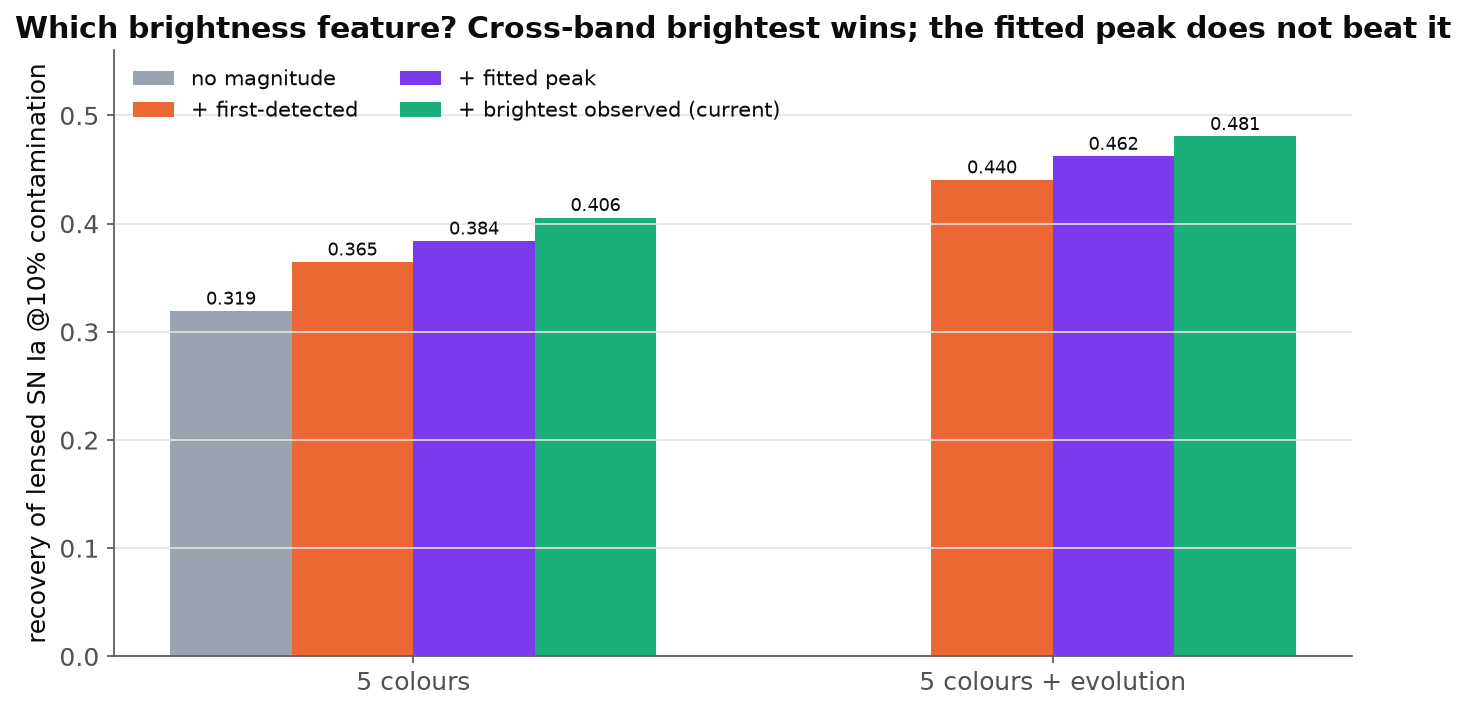
\includegraphics[width=\columnwidth]{peakmag_compare}
  \caption{Recovery of lensed SNe~Ia at 10\% contamination for three brightness
  features. A single-band fitted peak beats the first-detected magnitude but does
  not beat the cross-band brightest-observed sample, which is kept as the default.}
  \label{fig:magfeature}
\end{figure}

% =============================================================================
\section{Discussion}
\label{sec:discussion}

The results paint a consistent picture. Colour, framed as lensed SN~Ia versus the
full rate-weighted detected background, is a fast, cadence-robust early trigger:
it flags the majority of lensed SNe~Ia within days of first light and beats the
trailing image with weeks of lead. But it is fundamentally limited by two facts.
First, magnification is achromatic, so no colour feature can separate a lensed
from an unlensed SN~Ia; the $\sim$70\% unlensed-Ia detected background
(Section~\ref{sec:composition}) is irreducible by colour and sets the ceiling.
Second, at the true rarity of lensed SNe (Section~\ref{sec:baserate}) the flagged
sample is sub-percent pure. The trigger's proper role is therefore to hand a
short, early, ranked candidate list to a second, lensing-aware stage---light-curve
modelling, imaging for multiple images, and spectroscopy.

Several caveats bound the interpretation. The boundary-shape comparison
(Section~\ref{sec:gradient}) is fit on idealised model light curves, whereas the
multi-colour results put every class through a real cadence; a fully
cadence-consistent boundary study is a natural extension. The brightness feature
is settled empirically (Section~\ref{sec:magfeature}) rather than assumed, but a
multi-band, SED-aware peak fit could in principle improve on the brightest-observed
sample. Finally, our absolute purity and yield numbers inherit the uncertainties
of the adopted volumetric rates and lensed-SN forecasts; we have anchored these
to the literature but they remain the dominant systematic on the absolute scale,
not on the relative conclusions.

% =============================================================================
\section{Conclusions}
\label{sec:conclusions}

We have tested, end to end, whether colour alone can trigger on strongly lensed
SNe~Ia in LSST, with no host redshift and no spectroscopy. Our main conclusions
are:

\begin{enumerate}
  \item The optimal lensed/unlensed decision boundary is a smooth
  \emph{gradient}; candidates should be ranked by a calibrated probability, not
  hard-cut. Any flexible boundary lifts recovery from $\sim$0.63 (straight line)
  to $\sim$0.89.
  \item The flux-limited \emph{detected} background is SN\,Ia-dominated
  ($\sim$70\% unlensed Ia, $\sim$30\% CC), so the irreducible contaminant is the
  colour-identical unlensed SN~Ia.
  \item Under a real cadence the full colour vector is essential: one fixed colour
  recovers 11\% of lensed SNe~Ia at 10\% contamination, whereas using whatever
  bands are present recovers 32--48\%.
  \item The trigger flags 56\% of lensed SNe~Ia a median of $\sim$3\,d after first
  detection and beats the second image 85\% of the time by a median of 88\,d.
  \item At the true base rate the flagged sample is sub-percent pure: colour is a
  strong pre-filter ($\sim$40$\times$ cut in follow-up), not a standalone
  identifier.
  \item These conclusions are stable across the v5.3.2 and v5.3.5 OpSim baselines.
\end{enumerate}

Colour is therefore best deployed as the first, cheap stage of a multi-tier
lensed-SN discovery pipeline: an early, high-recall, ranked shortlist that a
lensing-aware follow-up stage can convert into confirmed systems in time to catch
the trailing images.

% =============================================================================
\section*{Acknowledgements}
We thank the Rubin Observatory and the LSST OpSim team for public cadence
simulations, and the developers of \textsc{sncosmo} \citep{Barbary2016},
\textsc{scikit-learn} \citep{Pedregosa2011}, \textsc{astropy}, \textsc{numpy}
and \textsc{matplotlib}. This work used the BlueBEAR HPC facility at the
University of Birmingham.

\section*{Data Availability}
The \textsc{cmsne} pipeline, the classifier, the analysis scripts, and a
demonstration notebook are available at
\url{https://github.com/anachoponte/Colour-Magnitude-SNe}. The OpSim cadence
databases are public Rubin Observatory data products.

% =============================================================================
\bibliographystyle{mnras}
\bibliography{references}

\bsp
\label{lastpage}
\end{document}
